% !TeX root = document.tex
% !TeX encoding = UTF-8 Unicode

\section{Introduction}%
\label{sec:introduction}

\subsection{Switched Systems}%
\label{subsec:switched-systems}

\begin{slide}{Switched Systems}
  \begin{columns}[c]
    \begin{column}{0.48\textwidth}
      \begin{itemize}
        \item A switched system is a system composed of many subsystems, called
              modes, and a mode-transition rule.
        \item Switched and switching systems are different in which the former
              is switched by a supervisor, whereas the latter switches
              arbitrarily.
      \end{itemize}
    \end{column}%
    \hfill%
    \begin{column}{0.48\textwidth}
      \begin{equation}
        \begin{aligned}
          \dot{x}(t) & = f_{\sigma(t)}(t,x(t),u(t)), \\
          y(t)       & = g_{\sigma(t)}(t,x(t)),
        \end{aligned}
      \end{equation}
      \vspace*{0.5cm}
      \begin{equation}
        \begin{aligned}
          \dot{x}(t) & = A_{\sigma(t)}x(t) + B_{\sigma(t)}u(t), \\
          y(t)       & = C_{\sigma(t)}x(t) + D_{\sigma(t)}u(t).
        \end{aligned}
      \end{equation}
    \end{column}%
  \end{columns}
\end{slide}

\begin{slide}{Switched Systems Stability Problem}
  \begin{columns}[c]
    \begin{column}{0.48\textwidth}
      \begin{itemize}
        \item The system can be stable under arbitrary switching.
        \item In case of nonlinear constraints (input or state) regional
              stabilization is required.
        \item Using Regional (or local) stabilization implies determining an
              estimate of the region of attraction.
      \end{itemize}
    \end{column}%
    \hfill%
    \begin{column}{0.48\textwidth}
      \begin{equation}
        \begin{aligned}
          A_{i}^{\top}P+PA_{i} & \prec{} 0 \\
          P                    & \succ 0
        \end{aligned}
      \end{equation}
      \begin{equation}
        Re = \{x\in R^n | x^\top P x \leq c,c>0\}
      \end{equation}
    \end{column}%
  \end{columns}
\end{slide}

\subsection{Command Governor}%
\label{subsec:cg}

\begin{slide}{Problem Description}
  \begin{columns}[c]
    \begin{column}{0.48\textwidth}
      How to keep the system's state and/or inputs constrained.
    \end{column}%
    \hfill%
    \begin{column}{0.48\textwidth}
      \begin{figure}[ht!]
  \centering
  \captionsetup{justification=centering}
  \begin{tikzpicture}[auto,node distance=1cm,>={Stealth},waypoint/.style={circle,inner sep=0pt,outer sep=0pt,thick},state/.style={circle,minimum size=1em,inner sep=0pt,outer sep=0pt},constraint/.style={ellipse,fill opacity=0.7,text opacity=1}]
    \node (x)  [state]                {\(\star\)};
    \node (w1) [waypoint,below=of x]  {};
    \node (w2) [waypoint,above=of x]  {};
    \node (w3) [waypoint,left=of x]  {};
    \node (a0) [waypoint,below left=3cm of x]   {};
    \node (a1) [waypoint,right=4cm of a0] {};
    \node (a2) [waypoint,above=4cm of a0] {};

    \begin{scope}[on background layer]
      \node (c1) [constraint,fill=cyan!80,fit=(w1) (w2) (w3)]    {};
    \end{scope}

    \draw [->] (a0) -- node [below] {\(x_{1}\)} (a1);
    \draw [->] (a0) -- node [left]  {\(x_{2}\)} (a2);
  \end{tikzpicture}%
  \caption{Constraint region and system's state}%
  \label{fig:dt-example}
\end{figure}

    \end{column}%
  \end{columns}
\end{slide}

\begin{slide}{Command Governor}
  \begin{columns}[c]
    \begin{column}{0.55\textwidth}
      % !TeX root = ../document.tex
% !TeX encoding = UTF-8 Unicode

\begin{figure}[ht!]
  \centering
  \captionsetup{justification=centering}
  % \resizebox{0.8\linewidth}{!}{%
  \begin{tikzpicture}[node distance=1cm,block/.style={align=center,draw,shape=rectangle,very thick,minimum height=2em, minimum width=3em},>={Stealth}]

    \node (r)  []                      {\(r(k)\)};
    \node (cg) [block, right=of r]     {Command\\Governor};
    \node (C)  [block, right=of cg]    {Primal\\Controller};
    \node (G)  [block, right=of C]     {System};
    \node (y)  [right=of G.north east] {\(y(k)\)};
    \node (c)  [right=of G.south east] {\(c(k)\)};
    \node (e)  [below=of C]            {\(\begin{bmatrix}x_{c}(k)\\x(k)\end{bmatrix}\)};
    \node [draw=blue,rectangle,dashed,fit=(C) (G) (e)] {};

    \draw [->, thick] (r) -- (cg);
    \draw [->, thick] (cg) -- node [above] {\(g(k)\)} (C);
    \draw [->, thick] (C) -- node (u) [above] {\(u(k)\)} (G);

    \draw [->, thick] ([yshift=-3mm]G.north east) -- (y.west);
    \draw [->, thick] ([yshift=3mm]G.south east) -- (c.west);
    \draw [->, thick] (G) |- node (x) [near start, above right] {\(x(k)\)} ([yshift=1em]e.south east);
    \draw [->, thick] (x) -| ([xshift=5mm]C.south);
    \draw [->, thick] (C) -- node [left] {\(x_{c}(k)\)} (e.north);
    \draw [->, thick] (e.west) -| (cg.south);
  \end{tikzpicture}%
  % }
  \caption{Command Governor Block Diagram.}%
  \label{fig:cg-schematic}
\end{figure}

    \end{column}%
    \hfill%
    \begin{column}{0.45\textwidth}
      \vspace*{0.5cm}
      \begin{equation}
        \begin{aligned}
          x(k+1) & = A_{i}x(k)+B_{i}u(k), \\
          y(k)   & = C_{i}x(k)+D_{i}u(k), \\
          c(k)   & = E_{i}x(k)+F_{i}u(k).
        \end{aligned}
      \end{equation}
      \begin{enumerate}
        \item \(\mathcal{C}\) is the set of restrictions.
        \item \(\mathcal{W} = \{\omega\in\mathbb{R}^{n_y}: c(k)\in\mathcal{C},k\rightarrow\infty{}\}.\)
        \item \(\mathcal{V}(x(k))=\{\omega\in\mathcal{W}:c(k)\in\mathcal{C},0<k\leq{}k_0\}.\)
      \end{enumerate}
      \vspace*{0.5cm}
      \begin{equation}
        \begin{aligned}
          g(k)=\argmin_{\omega\in\mathcal{V}(x(k))} & \norm{\omega-r(k)}^2_\Psi
        \end{aligned}
      \end{equation}
    \end{column}%
  \end{columns}
\end{slide}

\subsection{Supervisor}%
\label{subsec:supervisor}

\begin{slide}{Supervisor}
  \begin{columns}[T]
    \begin{column}{0.75\textwidth}
      \begin{figure}[ht!]
  \centering
  \captionsetup{justification=centering}
  \resizebox{!}{0.7\textheight}{%
    \begin{tikzpicture}[auto,node distance=1cm,>={Stealth},block/.style={draw,rectangle,minimum height=2em,minimum width=4em,thick},sum/.style={draw,circle,thick},point/.style={coordinate},dot/.style={draw,thick,circle,minimum size=0.5em},tight/.style={inner sep=0pt,outer sep=0pt}]
      \node (cg2) [block]              {\(CG_{2}\)};
      \node (C2)  [block,right=of cg2] {\(PC_{2}\)};
      \node (X2)  [tight,below=of C2]  {\(\begin{bmatrix}x_{C2}(k)\\x(k)\end{bmatrix}\)};
      \node [draw,rectangle,dashed,fit=(cg2) (C2) (X2)] {};
      \draw [->,thick] (cg2) -> node [below] {\(g_{2}(k)\)} (C2);
      \draw [->,thick] (C2) -> node [swap] {\(x_{C2}(k)\)} (X2);
      \draw [->,thick] (X2) -| (cg2);

      \node (cg3) [block,above=3cm of cg2] {\(CG_{3}\)};
      \node (C3)  [block,right=of cg3]     {\(PC_{3}\)};
      \node (X3)  [tight,below=of C3]      {\(\begin{bmatrix}x_{C3}(k)\\x(k)\end{bmatrix}\)};
      \node [draw,rectangle,dashed,fit=(cg3) (C3) (X3)] {};
      \draw [->,thick] (cg3) -> node [below] {\(g_{3}(k)\)} (C3);
      \draw [->,thick] (C3) -> node [swap] {\(x_{C3}(k)\)} (X3);
      \draw [->,thick] (X3) -| (cg3);

      \node (supervisor) [block,above left=of cg3,draw=orange] {Supervisor};
      \node (r) [left=of supervisor] {\(r(k)\)};
      \draw [->,thick] (supervisor) |- (cg2);
      \draw [->,thick] (supervisor) |- (cg3);

      \node (sw1) [tight,dot,right=2cm of C2]          {};
      \node (sw2) [tight,dot,above right=0.5em of sw1] {};
      \node (sw3) [tight,dot,below right=0.5em of sw1] {};
      \node (sw4) [point,right=1em of sw1]             {};
      \node (sw5) [point,right=1em of sw4]             {};
      \node (switch) [draw,rectangle,tight,fit=(sw1) (sw2) (sw3) (sw5),thick] {};
      \draw [thick] (sw5) -- (sw4) -- (sw2);

      \node (system) [block,right=1.5cm of switch] {System};
      \node (y) [right=of system] {\(y(k)\)};

      \draw [->,thick] (r) |- (supervisor);
      \draw [->,thick,dotted,draw=orange] ([yshift=0.75em]supervisor.south east) -| ([xshift=-0.5em]switch.north east);
      \draw [->,thick] (system) -- (y);
      \draw [->,thick,draw=blue] (switch) -- node {\(u_{i}(k)\)} (system);
      \draw [->,thick,draw=blue] (C3.east) -| node [below left] {\(u_{3}(k)\)} (sw2.north);
      \draw [->,thick,draw=blue] (C2.east) --  node {\(u_{2}(k)\)} (sw1.west);
      \draw [->,thick,draw=red] (system) |- node [above left] {\(x(k)\)} ([yshift=0.75em]X2.south east);
      \draw [->,thick,draw=red] (system) |- node [above left] {\(x(k)\)} ([yshift=0.75em]X3.south east);
      \draw [->,thick,draw=red] (system) |- ([yshift=-0.75em]supervisor.north east);
      \draw [->,thick,draw=red] (system) |- ++(-1cm,-1cm) -| ([xshift=-1em]C2.south east);
      \draw [->,thick,draw=red] (system) |- ++(-1cm,3cm)  -| ([xshift=-1em]C3.south east);
    \end{tikzpicture}%
  }%
  \caption{Supervisor Block Diagram.}%
  \label{fig:supervisor-schematic}
\end{figure}

    \end{column}%
    \hfill%
    \begin{column}{0.4\textwidth}
      \begin{figure}[ht!]
  \centering
  \captionsetup{justification=centering}
  \begin{tikzpicture}[auto,node distance=3cm,>={Stealth},waypoint/.style={draw,circle,minimum size=1em,inner sep=0pt,outer sep=0pt,thick},state/.style={draw,thick,circle,minimum size=1em,inner sep=0pt,outer sep=0pt},constraint/.style={ellipse,fill opacity=0.7,text opacity=1}]
    \node (x)  [state]                {\(\bullet\)};
    \node (w1) [waypoint,below=of x]  {\(\diamond\)};
    \node (w2) [waypoint,right=of w1] {\(\diamond\)};
    \node (w3) [waypoint,above=of w2] {\(\star\)};

    \begin{scope}[on background layer]
      \node (c1) [constraint,fill=cyan!80,fit=(x) (w1)]    {};
      \node (c2) [constraint,fill=green!80,fit=(w1) (w2)]  {};
      \node (c3) [constraint,fill=orange!80,fit=(w2) (w3)] {};
    \end{scope}

    \draw [->,thick] (x) -- (w1);
    \draw [->,thick] (w1) -- (w2);
    \draw [->,thick] (w2) -- (w3);
  \end{tikzpicture}%
  \caption{Supervisor Mode Management}
\end{figure}

    \end{column}%
  \end{columns}
\end{slide}

\subsection{Region of Attraction}%
\label{subsec:roa}

\begin{slide}{Poincaré-Bendixson's Theorem}
  \begin{figure}[!htb]
    \centering
    %
    \begin{subfigure}[b]{0.45\linewidth}
      \centering
      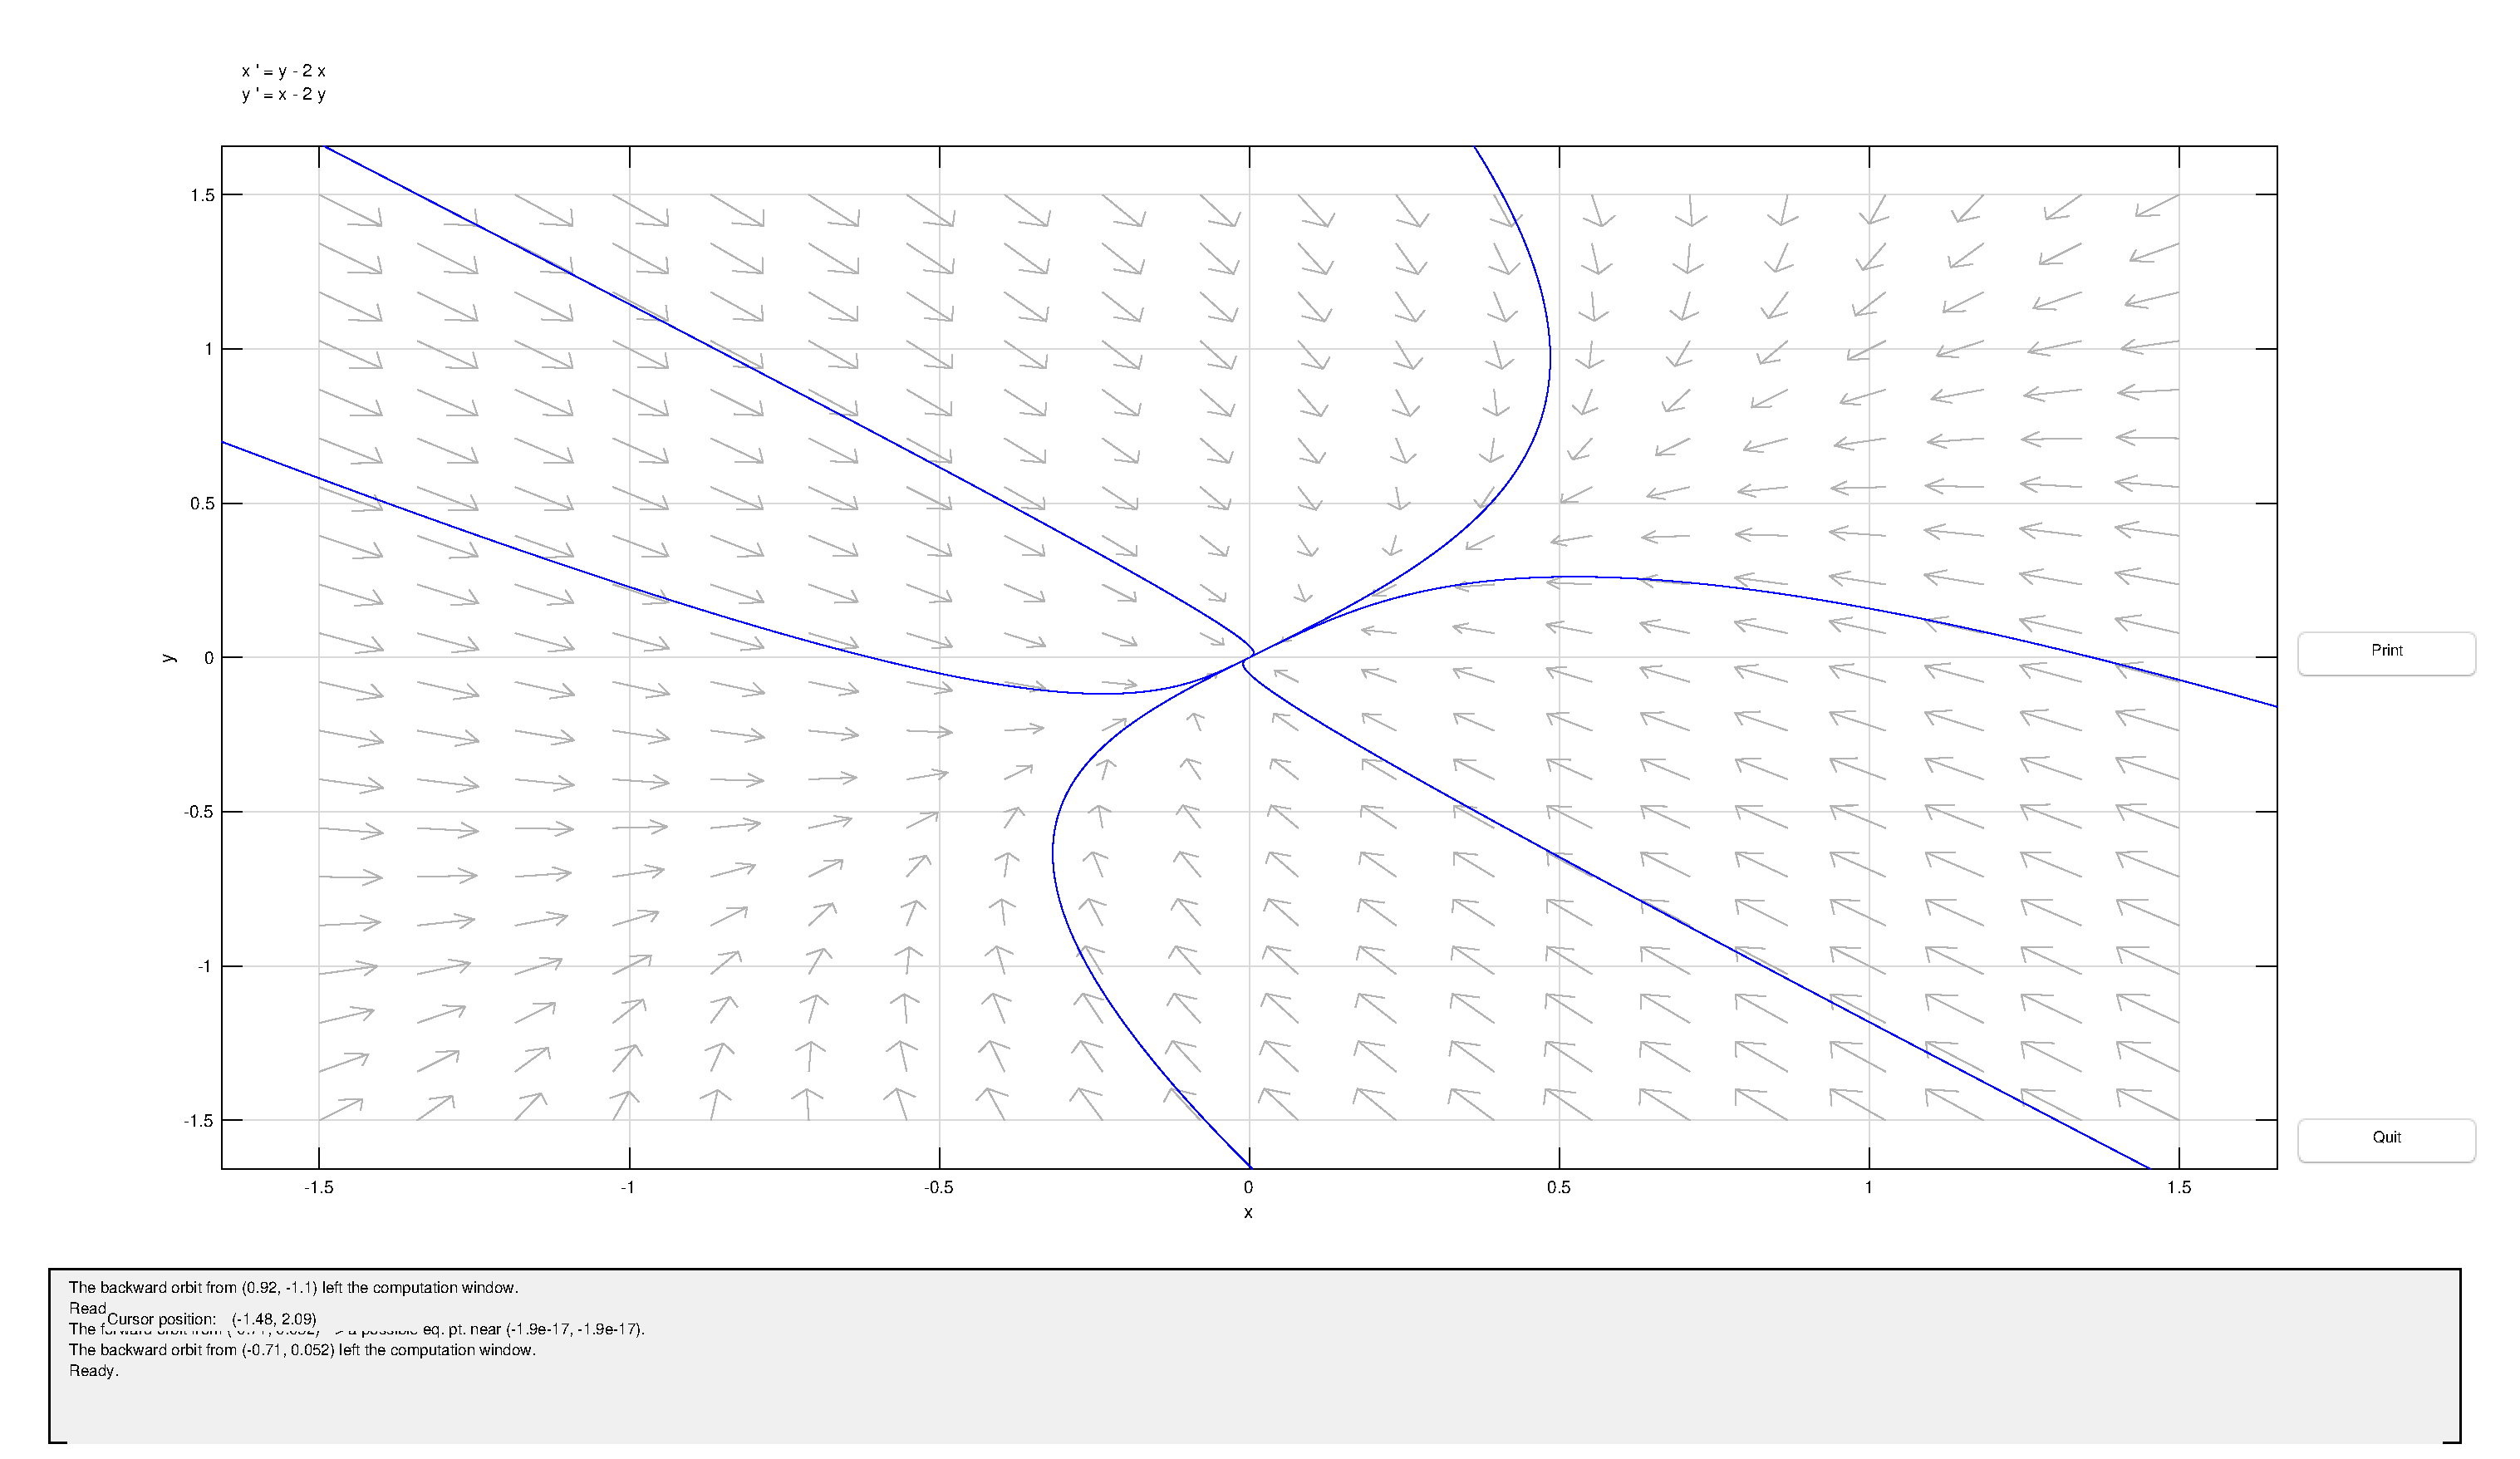
\includegraphics[trim=116 155 125 55,clip,width=\linewidth]{imgs/stable-point}
      \caption{Stable point}%
      \label{fig:stable-point}
    \end{subfigure}
    %
    \begin{subfigure}[b]{0.45\linewidth}
      \centering
      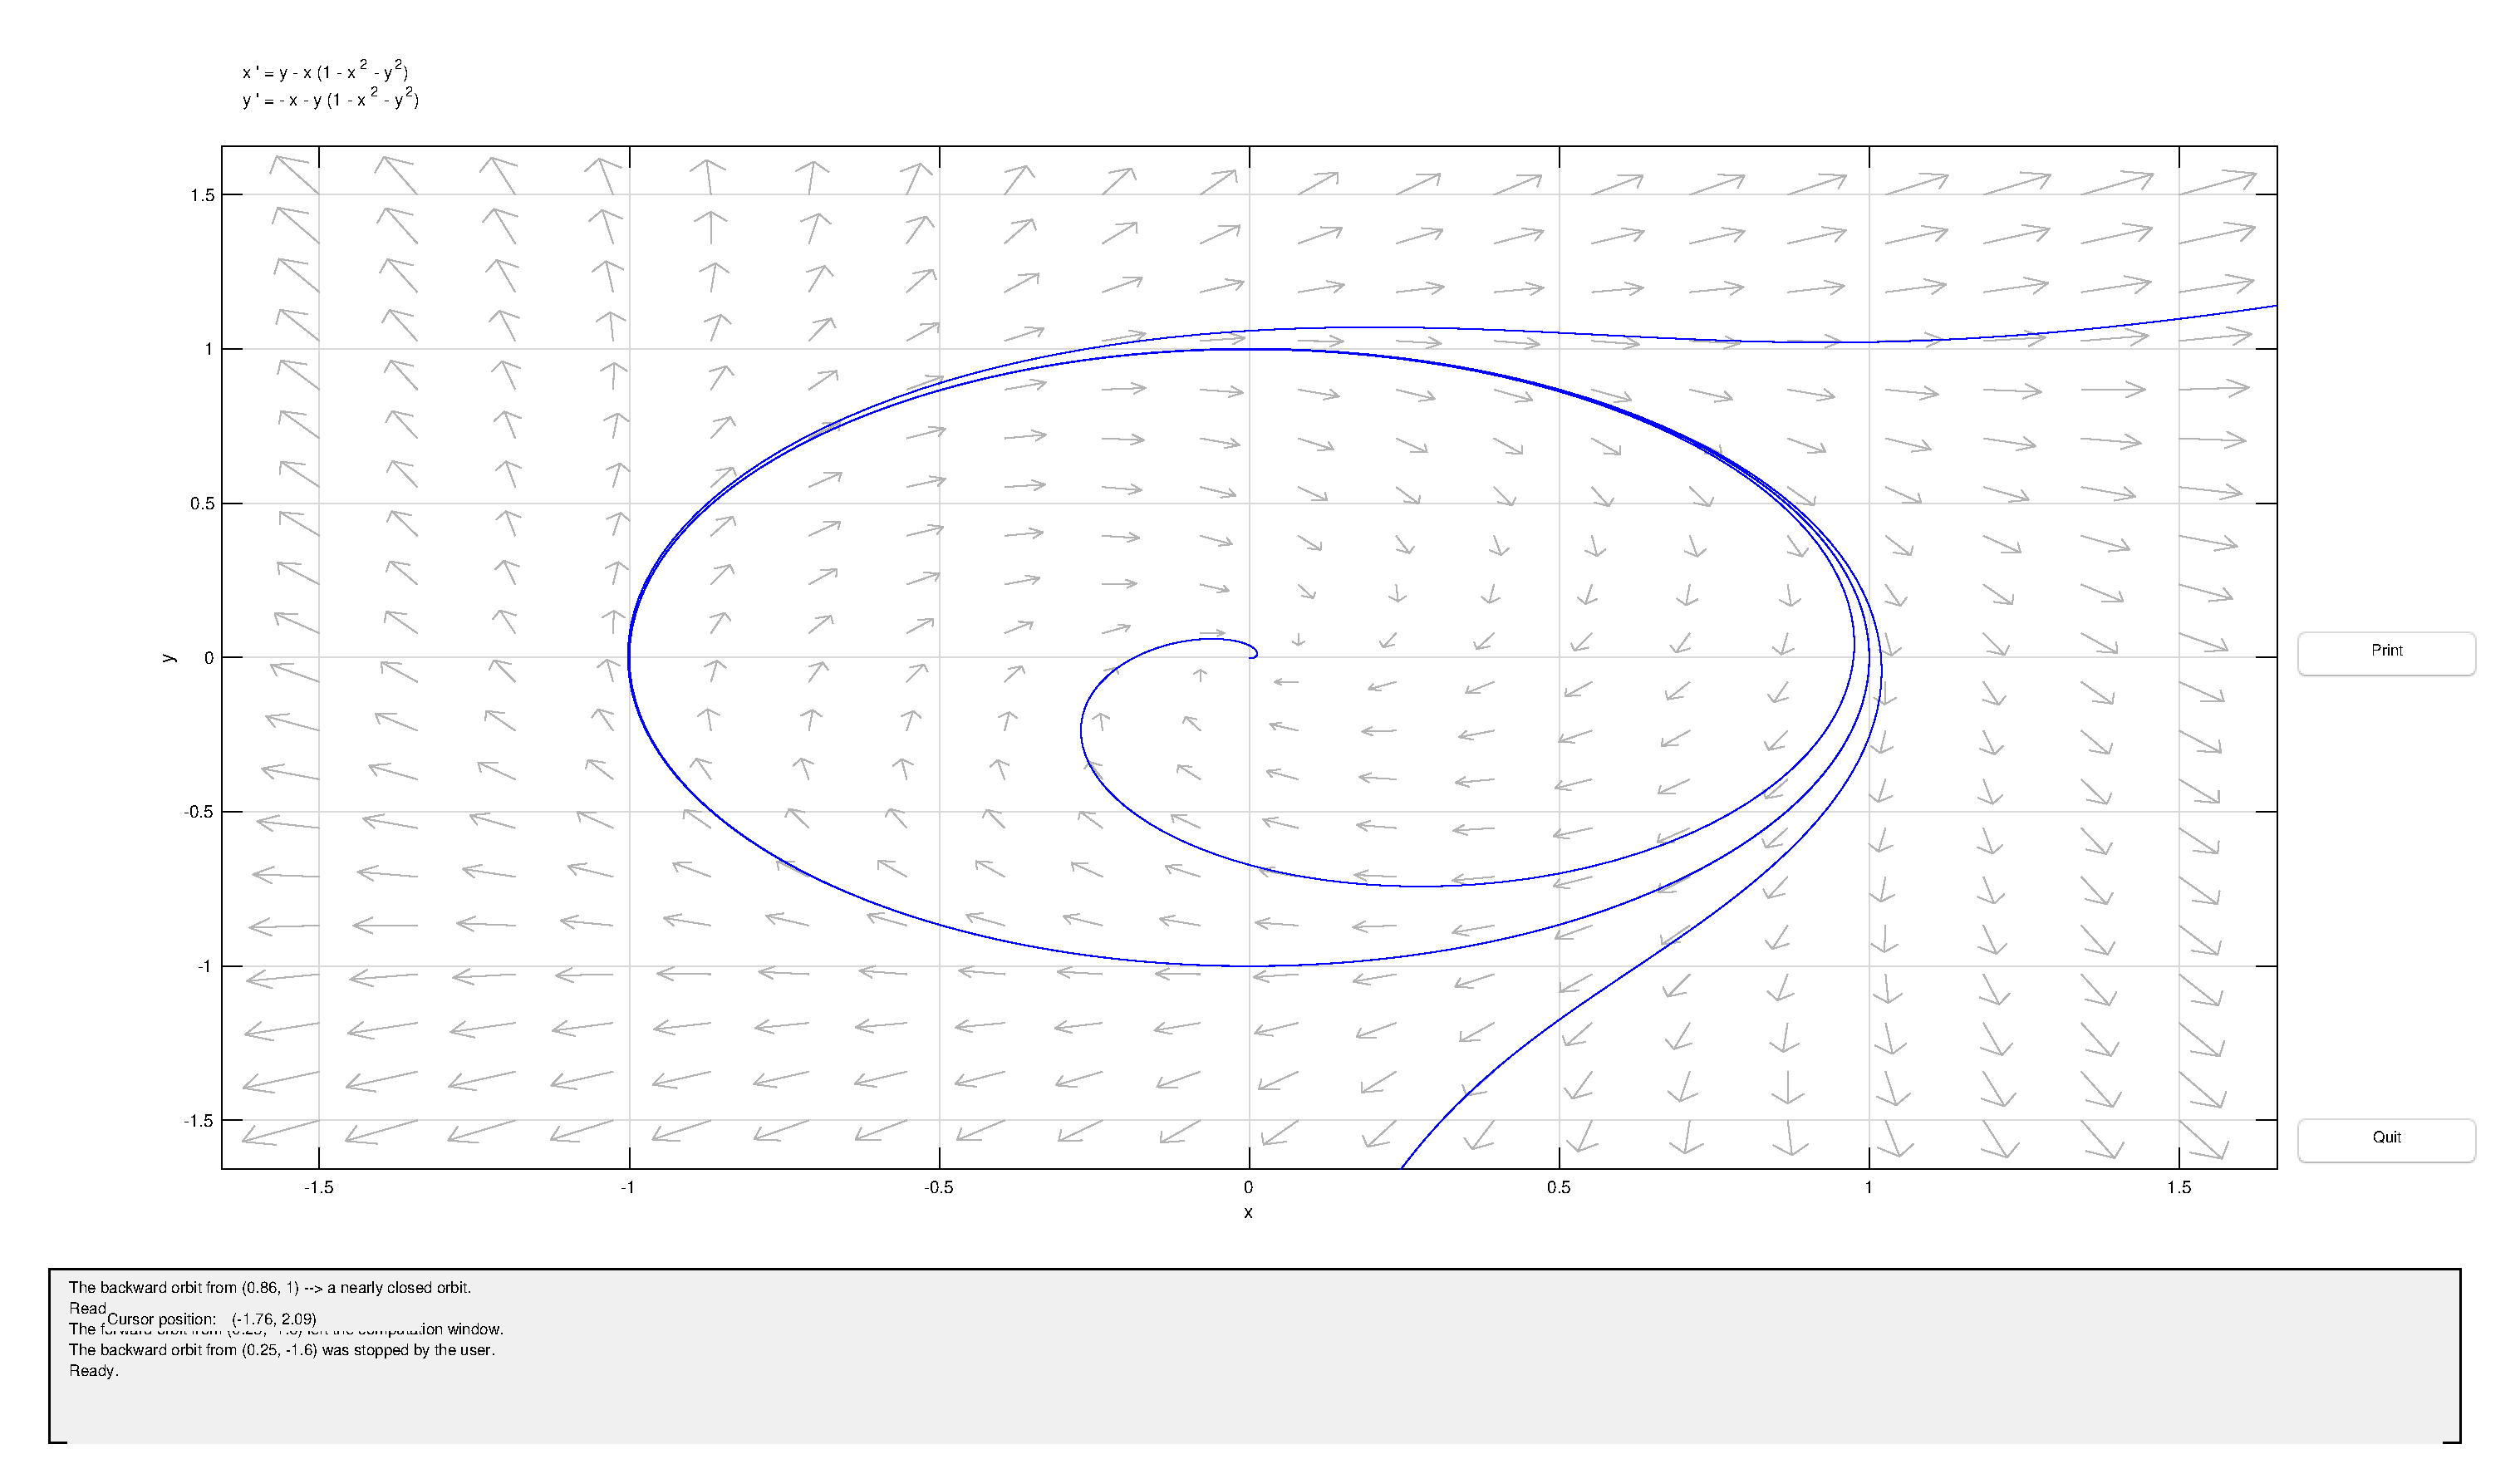
\includegraphics[trim=116 155 125 55,clip,width=\linewidth]{imgs/semi-stable-cycle}
      \caption{Semi-stable cycle}%
      \label{fig:semi-stable-cycle}
    \end{subfigure}
    %
    \caption{Different cycles' gradient maps}%
    \label{fig:poincare-cycles}
  \end{figure}
  \begin{equation}
    \nabla{}H(x)f(x) \leq 0
  \end{equation}
\end{slide}

\begin{slide}{Lyapunov's Theorem}
  \begin{equation}
    \begin{aligned}
      V(x)       & = 0 \iff x = 0,                                       \\
      V(x)       & > 0 \iff x \ne 0,                                     \\
      V(x_{1})   & > V(x_{2}) \iff \norm{x_{1}} > \norm{x_{2}},          \\
      \dot{V}(x) & = \nabla{}V(x)f(x) \le 0 \phantom{0} \forall x \ne 0.
    \end{aligned}
  \end{equation}
\end{slide}
